\section{Evaluation}
\label{sec:evaluation}

We distinguish implementation checks, reference and startup comparisons
at matched gains, and independently selected controllers. Reference calculations
are not counted as Callisto simulation runs. Appendix~\ref{app:evaluation}
contains the complete protocol, windows, replay diagnostics and
supplementary results.

\subsection{Plant, shared inputs and metrics}
\label{subsec:eval_design}
Callisto simulations retain continuous phases, integer frames, local
polling and delayed actuation. The nominal plant is a bidirectional
three-node triangle with six buffers, $C=2048$, initial/target
occupancy 1024 and initial phase 0.1. Uncontrolled frequencies are
\[
 \omega^u=(1.0002,0.9998,0.9999)^\top.
\]
Nominal physical link latency is 20;
the compatible initial in-flight count is 20 and marking is 1044.
Local polling/control delay are $p=1000$, $d_{\rm ctrl}=10$;
$h=p/\omega_{\rm base}$, $\omega_{\rm base}=29999/30000$.
Correction limit is 0.01; guards are enabled, reserve is zero and
anti-windup, observer and supervisory switching are disabled.

All candidates receive content-identical exogenous profiles per
comparison, with nominal prehistory. Disturbances begin at
$t_{\rm on}=2\times10^6$. Random desired latency is $20+z_m$ with
\begin{equation}
 z_0=5\varepsilon_0,\quad
 z_m=e^{-1}z_{m-1}+(1-e^{-1})5\varepsilon_m,
 \quad\varepsilon_m\sim\mathcal U[-1,1].
 \label{eq:eval_random_profile}
\end{equation}
Thus desired latency lies in $[15,25]$. The physical update grid
$T_c$ is independent of controller polling and is not an exactly
measured correlation time. Ordered running-maximum arrivals permit
batch release, without a finite serialization-rate model.

Let $\bar\omega=n^{-1}\sum_i\omega_i$ and define instantaneous
disagreement amplitude in parts per million (ppm) of unit frequency:
\begin{equation}
 s_\omega(t)=10^6\sqrt{n^{-1}\sum_i(\omega_i-\bar\omega)^2}.
\end{equation}
For a physical window $W$ of duration $T_W$, report
\begin{equation}
 R_W=\sqrt{T_W^{-1}\int_Ws_\omega^2dt},\quad
 I_W=\int_Ws_\omega dt,\quad P_W=\sup_Ws_\omega.
 \label{eq:eval_frequency_metrics}
\end{equation}
Here $I_W$ is RMS-amplitude integral absolute error (IAE).
Buffer excursion $B_W^{\rm obs}=\max_{e,t\in W}|\beta_e-\beta_e^*|$,
minimum two-sided headroom, mean per-node command total variation
(TV), common-frequency shift, saturation and gate events are separate
endpoints. Frequency moments use complete held intervals weighted by
physical duration; all integer crossings and ordered arrivals determine
buffer extrema. Display sampling is not used for peak statistics.
Window RMS alone does not certify pointwise pairwise spread.

Nominal centering requires three consecutive $10^5$-tick windows
before onset with RMS at most 2 ppm, each buffer's mean target bias
at most two frames and standard deviation at most one, common-frequency
standard deviation and three-window mean range at most 1 ppm,
positive progress and no intervention. Strict recovery additionally
requires a window-mean common frequency within 2 ppm of own clean,
the same-parameter nominal-delay counterfactual. Unobserved recovery
is right-censored. These are finite engineering criteria.

\subsection{Implementation and matched-gain safety evidence}
\label{subsec:eval_implementation_reference}
M0 consists of six PI/$F_0$ pairs (12 Callisto simulation runs), covering polling
100/1000, frequency spreads 35/400 ppm and capacity/target pairs
$(2048,1024)$, $(512,128)$ and $(512,384)$. Across 19800 updates,
maximum requested/applied correction difference is
$5.29\times10^{-18}$; phases, measurements and saved occupancies
agree without intervention. This validates PI calibration and
constructors, not full nonlinear superiority. Direct execution of
the original Fuzzy rules in the reference also agrees with the
17.314056818-frame peak and contraction checks. The all-time
guarantee still comes from the certificate, not finite simulation.

The reference safety sweep uses the fixed capacity, matched moderate
coordinates of Section~\ref{sec:btd_reference}, and
\begin{align}
 \omega^u(s)=\frac{29999}{30000}\mathbf1
                 +\frac{s}{30000}(7,-5,-2)^\top,\nonumber\\
 s\in\{0.5,1,2,4,8,16,32,64\}.
\end{align}
Its 32 trajectories cover both controllers and virtual/clipped
variants, with 2000 post-bootstrap intervals. Joint conditions hold
through common grid point $s=2$. At $s=4$ both trajectories are
observed-safe but uncertified; $s=32$ first requires clipping, and
the unprotected virtual buffers violate capacity at $s=64$.
The latter is not an actual guarded Callisto failure.

Before Callisto outcomes, the reference-based selection freezes
$s=2,4,32$. The six Callisto startup cases restore delay 20 and local
polling/control delay 1000/10, over $2001H\simeq2.001067\times10^6$
ticks. All retain positive frequency, capacity compliance and progress,
with zero replay mismatches/gate events. Initial negative history and
marking are reconstructed at each scale, including 21 in-flight frames
from the faster source at $s=32$.

\begin{table}[t]
\caption{Callisto startup stress at matched gains; extrema include all events.
Sat. counts saturated updates. These finite observations are not
certificates for delayed execution.}
\label{tab:eval_startup_safety}
\centering
\begin{tabular}{@{}rrrrr@{}}\toprule
 & & \multicolumn{2}{c}{Buffer excursion / frames} & Sat.\\
$s$ & Spread / ppm & PI & Fuzzy & PI / Fuzzy\\\midrule
2 & 800 & 47 & 37 & 0 / 0\\
4 & 1600 & 94 & 72 & 0 / 0\\
32 & 12800 & 750 & 664 & 176 / 85\\\bottomrule
\end{tabular}
\end{table}

Fuzzy reduces measured excursion at all three selected scales
(Table~\ref{tab:eval_startup_safety}). At 1600 ppm it decreases from
94 to 72 frames (23.4\%) without saturation, as
Figure~\ref{fig:eval_startup_actual} shows. This supports a conditional
headroom effect under the Callisto execution model. The 12800-ppm case
is a stress setting, not a typical hardware tolerance.

\begin{figure*}[t]
\centering
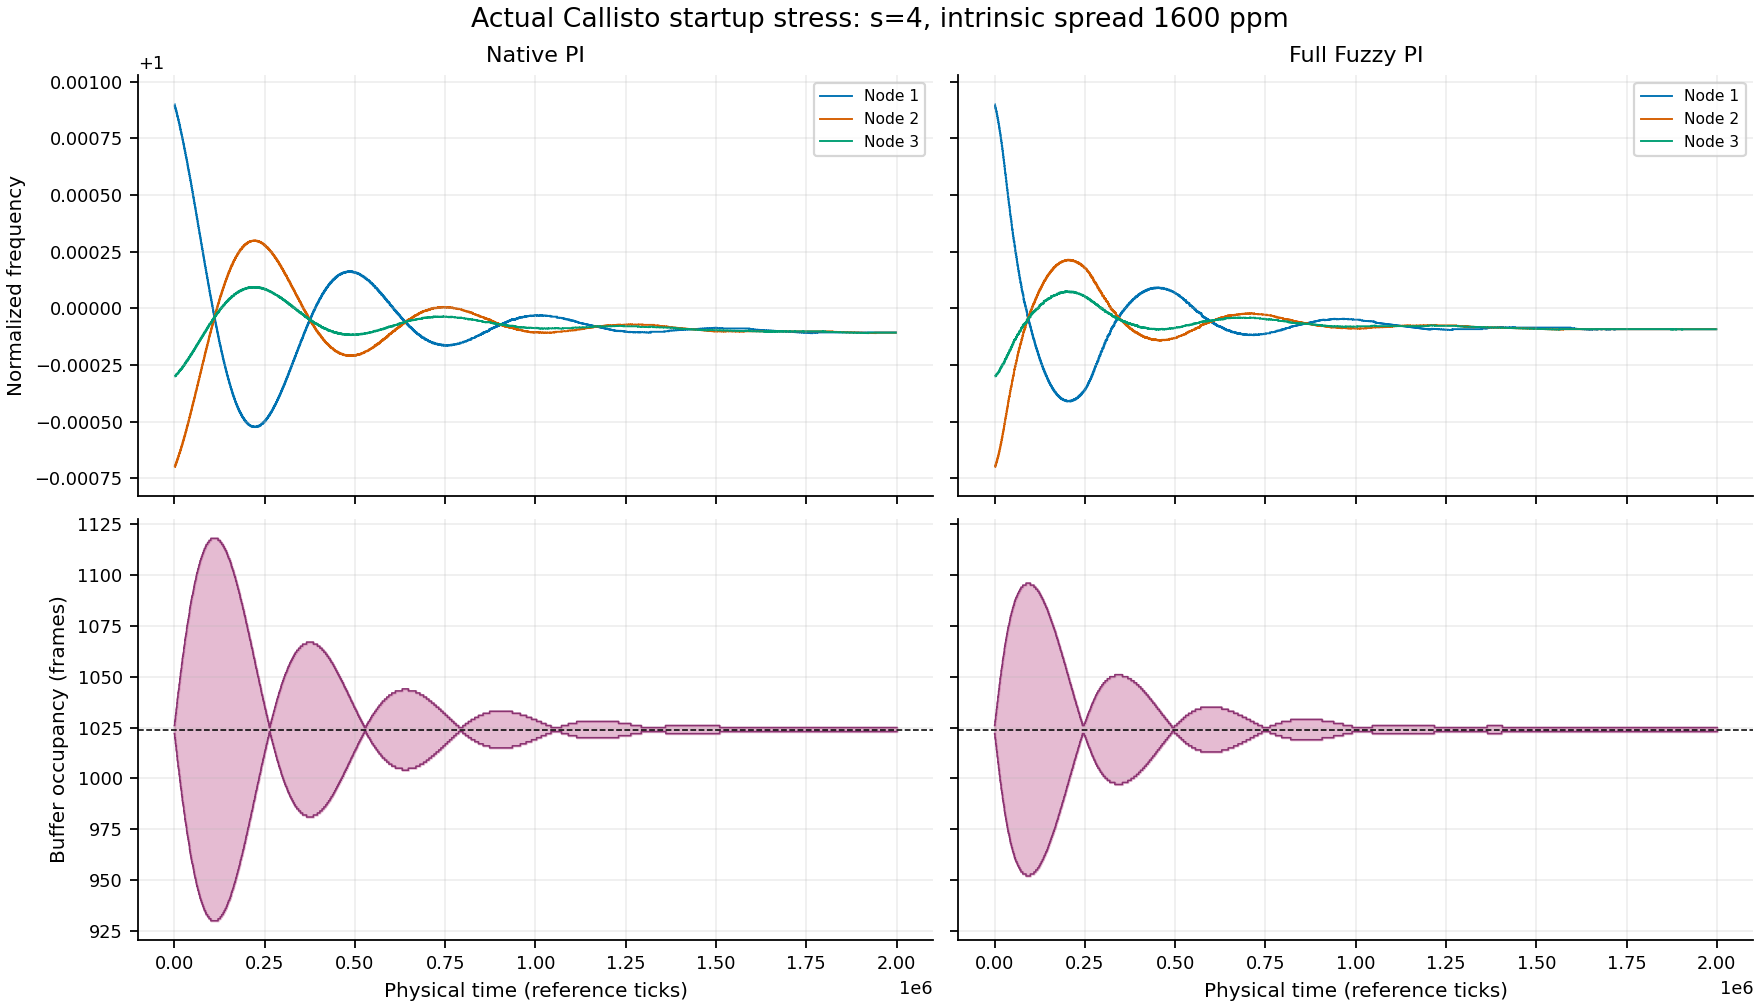
\includegraphics[width=0.94\textwidth]{images/evaluation_latest_20261103/actual_s4.png}
\caption{Callisto startup at 1600 ppm and matched moderate coordinates.
Upper panels show positive absolute frequencies with a $+1$ axis offset;
lower panels give the complete-event occupancy envelope across buffers.
Maximum deviation decreases from 94 to 72 frames.}
\Description{Matched PI and Fuzzy frequency and buffer transients at scale four.}
\label{fig:eval_startup_actual}
\end{figure*}

\subsection{Equal-budget selection and held-out random tests}
\label{subsec:eval_random}
Both families receive the same grid of 24 candidates:
\begin{align*}
 k_p&\in\{1.5,2,2.5,3,4,6\}\times10^{-6},\\
 k_i&\in\{1,2,5,10\}\times10^{-11}.
\end{align*}
Fuzzy fixes $K_e=0.1$;
the calibration determines its other scales, without an additional
shape-search dimension. Four training cases per candidate are clean,
a 20-tick single-edge delay increment lasting $10^5$ ticks, and
random $T_c=1000,10000$ with training seed 31001. All 192 slots
are charged, including four strictly verified cached evaluations;
188 are new Callisto simulation runs. Nineteen PI and 22 Fuzzy candidates pass
the same admissibility checks; seven infeasible candidates are retained.

The feasible Pareto set minimizes worst random RMS, burst IAE, worst
buffer excursion, peak absolute common-frequency excursion from
own clean and worst TV. Frozen lexicographic selection chooses random-
and burst-priority representatives, denoted $R$ and $B$. The selected
PI serves both priorities; Fuzzy selects two distinct representatives
(Table~\ref{tab:eval_selected_gains}). Gains and rules remain fixed
on tests; there is no online switching between them.

\begin{table}[t]
\caption{Frozen representatives in calibrated PI coordinates.
Fuzzy uses $K_e=0.1$ and~\eqref{eq:fpi_matching}. $R/B$ denote
random/burst selection priorities.}
\label{tab:eval_selected_gains}
\centering
\begin{tabular}{@{}llrr@{}}\toprule
Representative & Candidate & $k_p$ & $k_i$\\\midrule
PI$_R$=PI$_B$ & PI\_g05 & $2\times10^{-6}$ & $10^{-11}$\\
Fuzzy$_R$ & Fuzzy\_g02 & $1.5\times10^{-6}$ & $2\times10^{-11}$\\
Fuzzy$_B$ & Fuzzy\_g17 & $4\times10^{-6}$ & $10^{-11}$\\\bottomrule
\end{tabular}
\end{table}

Only after selection freezes are seeds 41001--41030 materialized.
All three candidates execute both random regimes and both held-out
bursts: $30\times2\times3+2\times3=186$ new Callisto simulation runs. All complete
and are normal-admissible, with no excluded seed pairs or engineering
QA errors. Earlier fixed-preset M2/M3 outcomes are development
evidence and never relabeled as these independent tests.

The registered random comparison is Fuzzy$_R$ versus PI$_R$. For
independent seed $\ell$, let $d_\ell=R_{W,\ell}^{\rm F}-R_{W,\ell}^{\rm PI}$
and $r_\ell=R_{W,\ell}^{\rm F}/R_{W,\ell}^{\rm PI}$.
Report their sample means, not a ratio of group means. Confidence
intervals use 20000 paired-seed percentile-bootstrap resamples, with
fixed seeds 58001/58002. Time points and edges are not replications.
Primary window is $W=[2\times10^6,4\times10^6)$; tail is
$[3.6\times10^6,4\times10^6)$. Nominal 97.5\% intervals per regime
also provide a two-regime Bonferroni adjustment.

\begin{table*}[t]
\caption{Held-out random-priority comparison: 30/30 admissible pairs per regime.
RMS entries are seed means in ppm; brackets are pointwise 95\% paired intervals.}
\label{tab:eval_random}
\centering
\begin{tabular}{@{}lrrll@{}}\toprule
Profile grid & PI$_R$ RMS & Fuzzy$_R$ RMS & Mean difference / ppm [CI] & Mean paired ratio [CI]\\\midrule
$T_c=1000$ & 4.61355 & 3.83949 & $-0.77406$ [$-0.80767$,$-0.73992$] & 0.83217 [0.82484,0.83964]\\
$T_c=10000$ & 4.65204 & 4.28718 & $-0.36486$ [$-0.43523$,$-0.29464$] & 0.92150 [0.90630,0.93672]\\\bottomrule
\end{tabular}
\end{table*}

Fuzzy's mean paired relative RMS improvements are 16.78\% and 7.85\%
(Table~\ref{tab:eval_random}, Figure~\ref{fig:eval_random_primary}).
The family-adjusted difference intervals also lie below zero:
$[-0.81274,-0.73483]$ and $[-0.44451,-0.28407]$ ppm.
This establishes a selected-scheme advantage within the finite grid
and two input regimes, not a same-gain inference-only effect or
global controller optimality.

\begin{figure*}[t]
\centering
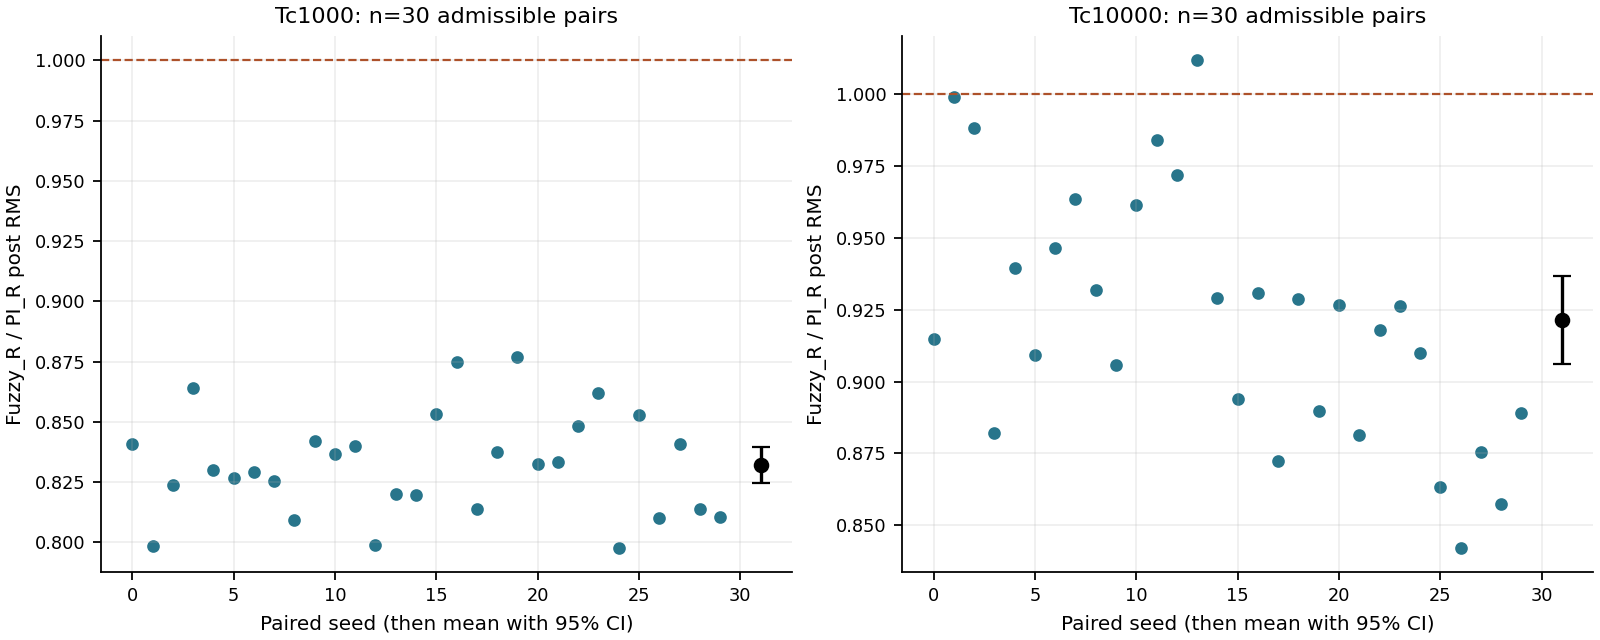
\includegraphics[width=0.94\textwidth]{images/evaluation_latest_20261103/paired_random_effects.png}
\caption{Held-out paired Fuzzy$_R$/PI$_R$ RMS effects. Dots are independent
seed pairs; the black marker gives the mean paired ratio and pointwise
95\% CI. The dashed line denotes equal RMS.}
\Description{Thirty seed-level ratios and aggregate effects in each original regime.}
\label{fig:eval_random_primary}
\end{figure*}

Mean TV also decreases: 0.0102361 to 0.00782282 at $T_c=1000$,
and 0.00112361 to 0.000906694 at $T_c=10000$ (PI to Fuzzy).
All selected candidates have at most six frames of disturbance-window
buffer deviation. The benefit carries a common-frequency cost:
mean own-clean tail shifts are $-61.420$ versus $-15.692$ ppm,
and $-31.933$ versus $-15.384$ ppm (Fuzzy versus PI). Relative
agreement and absolute-rate tracking are different objectives.

\begin{figure*}[t]
\centering
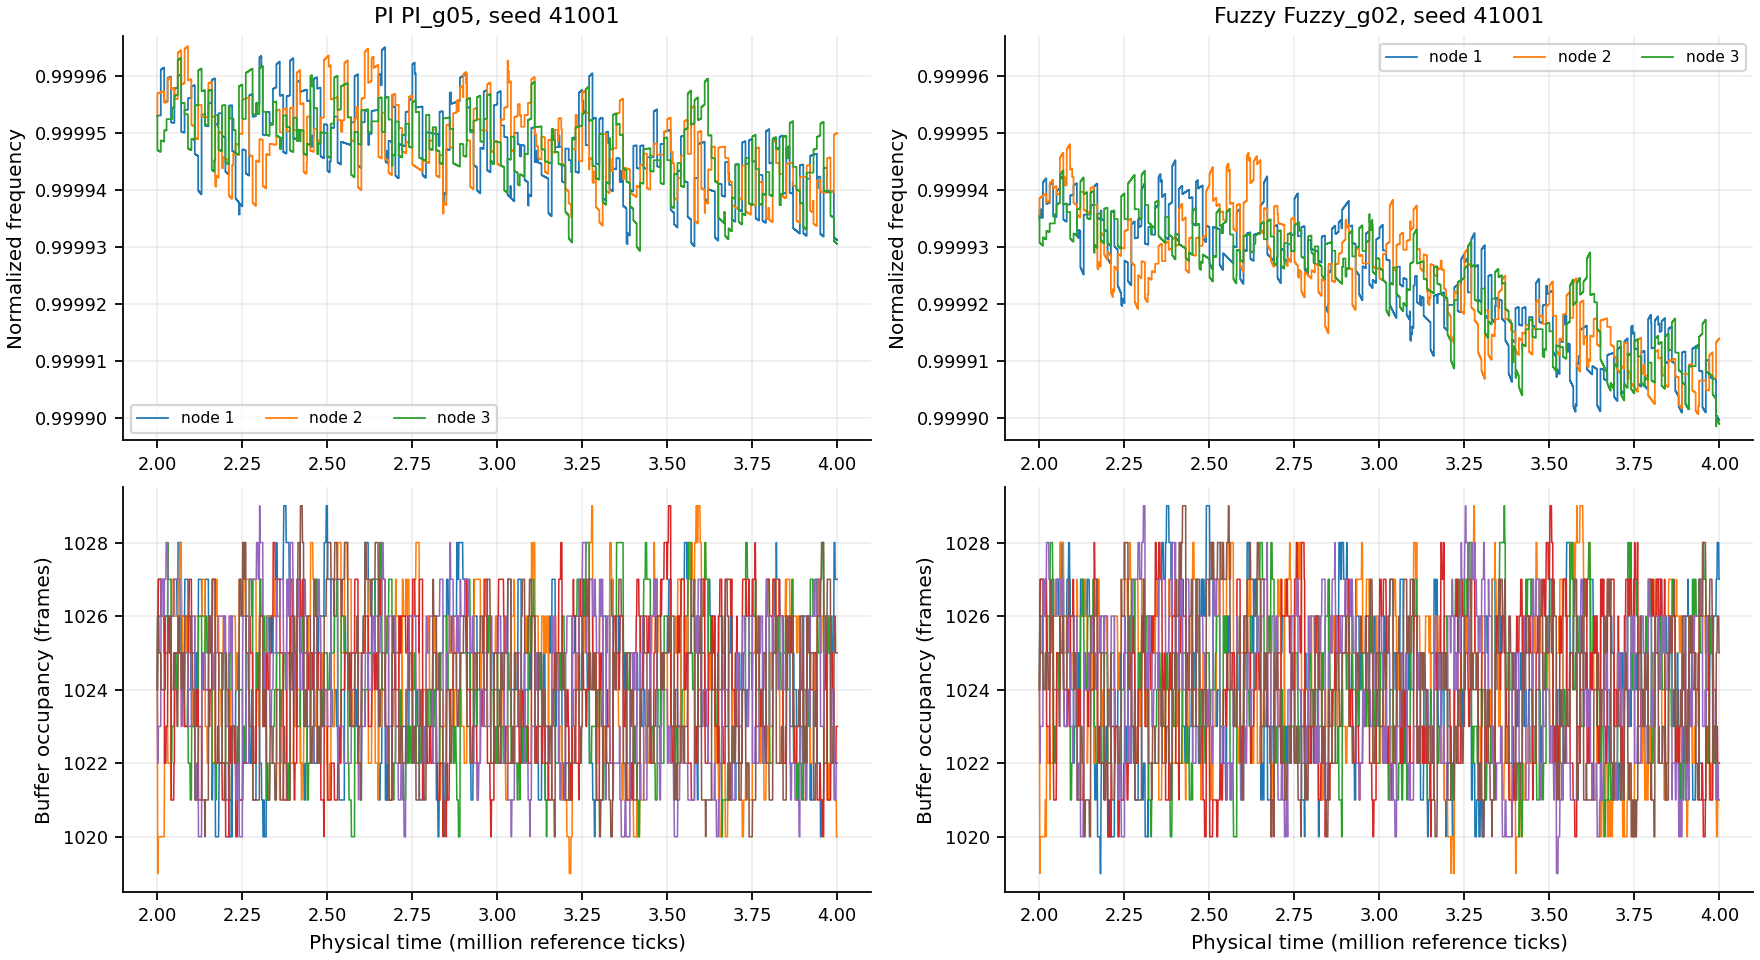
\includegraphics[width=0.94\textwidth]{images/evaluation_latest_20261103/raw_Tc10000.png}
\caption{Raw response for the first held-out seed (41001), $T_c=10000$.
Frequency uses held corrections and a common physical axis. Buffer curves
show saved occupancies; complete-event replay supplies reported extrema.
The different common-frequency shifts are visible independently of
relative disagreement. This one trace illustrates the experiment;
the 30 paired seeds support the statistical comparison.}
\Description{Raw node frequencies and receiving-buffer occupancies for the same held-out random profile.}
\label{fig:eval_random_raw}
\end{figure*}

Figure~\ref{fig:eval_random_raw} retains raw curves rather than only
aggregate scores. The controls see their own local buffers and hence
generate different subsequent schedules even under identical external
profiles. Comparing saved sample indices or one node's update count
would therefore misalign physical times. Shared physical intervals,
own-clean histories and complete-event peaks are needed to assess
the actual transient. The displayed seed is the first by identifier,
not selected for the largest improvement. The small post-onset
occupancy excursions also show why these random runs alone cannot
establish a larger safe set: both controllers operate far from capacity.

\paragraph{Selection and evaluation answer different questions.}
Training contains one seed per regime, so its objective values define
a fixed-input search criterion, not population effect estimates.
The five objectives are retained separately rather than combined
with post hoc weights. The $R$ ordering prioritizes worst random RMS,
then common excursion, buffer excursion, burst IAE and TV; $B$
prioritizes burst IAE, then buffer excursion, common excursion,
random RMS and TV. Candidate identifiers break exact ties.
Publishing both selected Fuzzy representatives avoids presenting the
random-priority candidate as the best design for every task. All
representatives nevertheless execute all held-out inputs. These
choices keep the favorable random comparison distinct from selecting
a winner after seeing independent outcomes.

\subsection{Burst validation and operating limits}
\label{subsec:eval_burst}
The held-out combinations are a 10-tick desired delay increment
lasting $10^4$ ticks on $2\to3$, and a 40-tick increment lasting
$10^5$ ticks on $3\to1$. They are not training combinations.
For the larger burst Fuzzy$_B$ reduces IAE by 55.8\% while retaining
the same buffer peak; the smaller case limits generalization
(Table~\ref{tab:eval_heldout_bursts}). Deterministic cases do not
supply seed-level confidence intervals.

\begin{table}[t]
\caption{Both held-out burst-priority cases. IAE is in $10^6$
ppm$\cdot$ticks; excursion is in frames, over the same post-onset window.
$A,D$ are delay increment and duration.}
\label{tab:eval_heldout_bursts}
\centering
\begin{tabular}{@{}lrrrr@{}}\toprule
 & \multicolumn{2}{c}{IAE} & \multicolumn{2}{c}{Buffer excursion}\\
Case & PI$_B$ & Fuzzy$_B$ & PI$_B$ & Fuzzy$_B$\\\midrule
$A=10,D=10^4$ & 0.265814 & 0.352614 & 11 & 11\\
$A=40,D=10^5$ & 8.192410 & 3.623166 & 40 & 40\\\bottomrule
\end{tabular}
\end{table}

A separate slower-delivery study retains all selected gains. Four
ramp--hold--ramp combinations use rise/fall times $10^4/10^5$ and
hold times $10^5/10^6$, a 20-tick increment on $1\to2$, horizon
$5.2\times10^6$ and two million ticks of recovery after each fall.
At the slower rise, buffer peaks are PI 19, Fuzzy$_R$ 18 and
Fuzzy$_B$ 17 frames; frequency RMS favors PI. Strict own-clean
recovery is censored in all 12 ramp cases. Holding high latency
does not stop delivery for the entire plateau; ramping instead
permits feedback while the imbalance forms.

For slow random $T_c=100000$, 30 new seeds 51001--51030 use
an observation window from $2\times10^6$ to $5\times10^6$ ticks.
The paired RMS ratio is 1.33312
[1.30337,1.36219], delimiting the original-regime advantage.
The complete slower study contains 105 matrix slots, four reused
pilot slots and 107 unique Callisto simulation runs including six pilots; all
event-replay and nominal checks pass. Profile blocks are not
independent replications. Supplementary traces, protocols and
effects are retained in Appendix~\ref{app:evaluation}.

Finally, all 299 new validation/slow-delivery/startup raw records
pass controller reconstruction, with maximum requested-output
residual $5.42\times10^{-20}$. The M2 mechanism trace remains in
$\Omega_5$, but selected Fuzzy$_B$ reaches input-diamond peak
39.159 in the large burst. The full rule law executes there;
the central identity and $\Omega_1$ witness do not cover that trace.
Finite-time simulation compliance does not transfer the reference
all-time guarantee or establish a generally enlarged safe set.
